\section{Simulation}

\subsection{Motivation für Simulationen}
\begin{itemize}
	\item Das Verhalten kann mittels Simulationen analysiert werden
	\item Mit Simulationen können Zeiten verkürzt werden
	\item Durch Simulationen kann die Reaktion der Steuerung auf Ausnahmesituationen überprüft werden
\end{itemize}

\subsection{Vernünftige Eingabewerte}
Ablauf einer Simulation: Einem Simulator werden vernünftige Eingabewerte gegeben und seine Reaktion darauf überprüft.
\subsubsection{Reale Eingabewerte für Simulatoren}
\begin{itemize}
	\item Reale, "'vernünftige"' Eingabewerte entsprechen möglichst gut der Realität
	\item Häufig sollen bei Simulationen zufällige Eingabewerte verwendet werden, die nicht notwendigerweise gleichverteilt sind. Häufig vorkommende Verteilungen sind:
	  \begin{itemize}
	    \item Gleichverteilung
		\item Normalverteilung (Gauss'sche Glockenkurve)
		\item Rayleigh-Verteilung
		\item Weibull-Verteilung
	  \end{itemize}
	\item Die Simulationen sollen reproduzierbar sein.
\end{itemize}

\subsection{Zufallszahlen-Generator (Random Number Generator, RNG)}
\subsubsection{Zufallszahlen}
\begin{itemize}
	\item Echt zufällige Zahlen können nur durch einen physikalischen Prozess erzeugt werden, z.B. durch Würfel oder Thermisches Rauschen.
	\item Eine deterministische Maschine wie der Computer kann keine echt zufälligen Zahlen generieren (ausser mit zusätzlicher Hardware $\rightarrow$ siehe TRNG).
	\item Ein Computer kann immerhin pseudozufällige Zahlen liefern.
\end{itemize}

\subsection{Pseudozufallszahlen-Generator}
\subsubsection{Pseudozufällige Zahlen}
\begin{itemize}
	\item Pseudozufällige Zahlen sind deterministisch. Bei einem gegebenen Anfangswert (random seed) und gegebener Zufallszahlenfunktion ist die zufällige Zahlenfolge immer identisch. $\rightarrow$ hat den Vorteil, dass eine Simulation reproduzierbar wird.
	\item Der Nachteil ist, dass keine wirklich zufälligen Zahlen entstehen. Durch eine intelligent gewählte Funktion kann jedoch eine sehr hohe Periode der Folge erreicht werden, auch das Erraten der nächsten Zahl ist ohne Kenntnis des Random Seeds und der Funktion beinahe unmöglich.
	\item Für kryptographische Anwendungen braucht es einen True Random Number Generator (TRNG), ein Pseudo RNG genügt nicht.
\end{itemize}

\subsubsection{Forderungen}
\begin{itemize}
	\item Gleichverteilung
	\item Nächste Zahl nicht vorhersehbar
\end{itemize}

\subsubsection{Methoden}
\begin{itemize}
    \item Lineare Kongruenz: $r_{i+1} = (a \cdot r_i + c)\cdot mod (m)$
    \item Multiplikative Kongruenz (c=0): $r_{i+1} = (a \cdot r_i)\cdot mod (m)$
\end{itemize}

\subsubsection{rand() und srand()}
\begin{itemize}
    \item \lstinline{int rand(void); // not thread-safe} $\rightarrow$ liefert gleichverteilte Zahlen im Bereich von [0, RAND\_MAX]
    \item \lstinline{void srand(unsigned int seed);} $\rightarrow$ setzt den Anfangswert, den random seed ($r_0$)
		\item \lstinline{int rand_r(unsigned int* seedp); // thread-safe (check man pages)}
\end{itemize}
Beispiel:
\lstinputlisting[language=C++]{code/srand.cpp}

\subsubsection{Mapping von Zufallszahlen auf beliebige Bereiche}
rand() = Gleichverteilung\\

\begin{tabular}{|l|l|}
	\hline
	\textbf{rand()} & Liefert ganzzahlige Werte im Bereich [0, RAND\_MAX] \\
	\hline
	\textbf{rand() \% n} & Liefert Werte im Bereich [0, n-1] \\
	\hline
	\textbf{(double)rand()/RAND\_MAX} & Liefert Werte im Bereich [0.0, 1.0] \\
	\hline
	\textbf{(double)rand()/RAND\_MAX$\cdot$(b-a) + a} & Liefert Werte im Bereich [a, b] \\
	\hline
\end{tabular} \\\\

\textbf{Bei einer Umwandlung in eine ganze Zahl muss beachtet werden, ob runden oder abschneiden die richtige Operation ist.}\\

Dies ist speziell dann wichtig, wenn die Verteilung positive und negative Zahlen beinhalten soll. Bei Truncating  (Abschneiden) (einfacher (int)-Type-Cast) würden dabei bei 0 doppelt so viele Werte sein, weil alle Werte innerhalb ]-1.0, 1.0[ auf 0 abgeschnitten würden.

\subsubsection{Gleichverteilung von ganzen Zahlen in [low, high]}
\begin{lstlisting}
static_cast<int>(static_cast<double>(rand()) / (RAND_MAX + 1.0) * (high-low + 1)) + low
\end{lstlisting}
\begin{itemize}
  \item (RAND\_MAX + 1.0) ist notwendig, damit 0.0  $\leq$ u $<$ 1.0 (ohne 1.0) erzeugt wird. (RAND\_MAX + 1) gäbe einen int-Overflow
  \item (high – low + 1) ist notwendig, weil nach int konvertiert wird. Vor der int-Konversion gibt es dadurch bei [1,20] Zahlen im Bereich [0.0, 20.0[. Nach der Konversion werden nur die ganzzahligen Anteile verwendet.
  \item Das hinterste + low muss ausserhalb des Typecasts sein, andernfalls ergibt es eine Überhöhung bei 0, falls low $<$ 0 (alle Zahlen in ]-1.0, +1.0[ würden zu 0, d.h. doppelt so viele wie erlaubt)
	\item Aber: Division ist immer noch drin
\end{itemize}

\textbf{Ohne Division:}

\begin{itemize}
	\item Ansatz:
	\begin{itemize}
		\item Der Bereich [0, RAND\_MAX] wird in (high - low + 1) gleiche Teile aufgeteilt.
		\item Falls der Zufallswert im untersten Bereich liegt, ergibt dies low, im zweituntersten low + 1 usw., der oberste Bereich ergibt high.
	\end{itemize}
	\item Dadurch werden Divisoren vermieden. Stattdessen gibt es Fallunterscheidungen. Diese sind häufig effizienter.
	\item Bei Mikrocontrollern mit Pipelines muss allerdings beachtet werden, dass Fallunterscheidungen potentiell zu pipeline flushes führen können.
	\item Für einen Bitstream wird die Implementation trivial: \lstinline{bit = rand() <= RAND_MAX/2? 0: 1;}
\end{itemize}

\subsection{Hardware True RNG (TRNG)}

\subsubsection{Einschränkungen des Pseudo RNG}
\begin{itemize}
	\item Wenn der Random Seed und die Formel bekannt ist, kann die ganze Folge eruiert werden.
	\item Pseudo RNGs sind deterministisch
	\item RNGs werden häufig bei kryptographischen Verfahren eingesetzt
	\begin{itemize}
		\item Schlüsselgeneration, Challenge-Response, etc.
	\end{itemize}
	\item Unzuverlässige, bzw. nachvollziehbare RNGs sind eine gute Gelegenheit für Hacker
	\begin{itemize}
		\item Schlüssel können vorhergesagt werden
		\item Challenges können allenfalls über eine gewisse Zeit repetiert werden
		\item Mischen bei Glücksspielen kann vorhergesagt werden
	\end{itemize}
	\item PRNGs genügen praktisch immer, ausser in kryptographischen Anwendungen
\end{itemize}

\subsubsection{kryptographisch sichere PRNG (CSPRNG)}
\begin{itemize}
	\item Eine CSPRNG hat zwei Eigenschaften zu erfüllen:
	\begin{itemize}
		\item Es ist nicht möglich, aus n Bits eines Schlüsselstroms das nächste Bit zu ermitteln.
		\item Es ist nicht möglich, aus n Bits eines Schlüsselstroms das vorherige Bit zu ermitteln.
	\end{itemize}
	\item Die genauere Definition besagt, dass es keinen Algorithmus mit polynomialer Laufzeit gibt, der das Bit $s_{i+n}$ mit einer Wahrscheinlichkeit von mehr als 50\% plus einer vernachlässigbar kleinen Abweichung berechnen kann.
\end{itemize}

\subsubsection{True Random Number Generators (TRNG)}
\begin{itemize}
	\item TRNGs produzieren Zahlen aus einem physikalischen Prozess, z.B.
	\begin{itemize}
		\item einem Münzwurf
		\item Würfeln
		\item Thermisches Rauschen eines Halbleiters
		\item Takt-Jitter elektronischer Schaltungen
		\item Radioaktivem Zerfall, etc.
	\end{itemize}
	\item Es gibt verschiedene ASICs, die TRNGs liefern und auch in Computersystemen eingesetzt werden können.
\end{itemize}

\subsubsection{Hardware RNG (True RNG): Bull Mountain (Intel\textsuperscript{\textregistered} Secure Key)}

\begin{itemize}
    \item Clock = LOW: Transistoren leiten und zwingen Node A und B auf Vcc
    \item Clock = rising edge: Transistoren sperren
    \item Node A und B pendeln sich auf eine mittlere Spannung ein, bevor sie aufgrund von thermischem Rauschen zufällig auf 0 oder 1 fallen (jeweils invertiert)
\end{itemize}

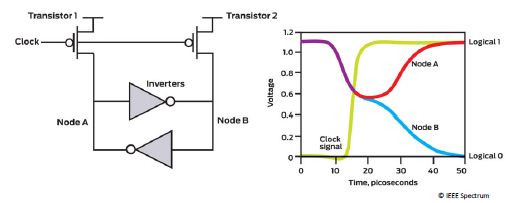
\includegraphics[width=0.7\textwidth]{images/Simulation/TRNG.png}

\subsection{Erzeugung beliebiger Verteilungen}
\subsubsection{Normal-/Gaussverteilung}
\begin{itemize}
    \item Kommt sehr häufig in der Praxis vor (Natur, Ingenieurwesen, Wirtschaft, etc.)
        \begin{itemize}
            \item Zufällige Messfehler um einen Sollwert
            \item Fertigungsschwankungen um einen Sollwert
        \end{itemize}
    \item Charakterisierung durch Mittelwert $\mu$ (häufigster Wert, Erwartungswert) und Standardabweichung $\sigma$  (Mass für Streuung, Breite der Glockenkurve)
    \item Eigenschaften der Normalverteilung:
        \begin{itemize}
            \item 68 \% aller Werte liegen innerhalb von $\mu \pm \sigma$
            \item 95 \% aller Werte liegen innerhalb von $\mu \pm 2\sigma$
            \item 99.7 \% aller Werte liegen innerhalb von $\mu \pm 3\sigma$
            \item 99.99 \% aller Werte liegen innerhalb von $\mu \pm 4\sigma$
        \end{itemize}
    \end{itemize}
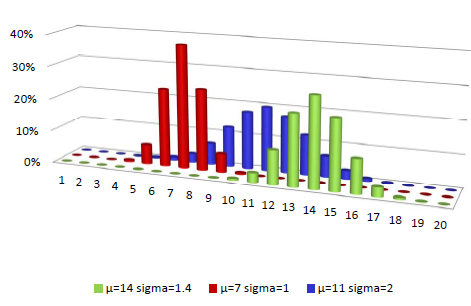
\includegraphics[width=0.5\textwidth]{images/Simulation/Normalverteilung.png}\\\\
\textbf{Zentraler Grenzwertsatz}\\
Die Summe von n unabhängigen, identisch verteilten Zufallszahlen stellt für n gegen unendlich eine Normalverteilung dar. \\\\ Eine Normalverteilung kann somit angenähert werden, wenn eine grosse Anzahl gleichverteilter Zahlen summiert wird. Die einfachste Methode ist die \textbf{Polarmethode von Marsaglia} (basiert auf Box-Muller-Algorithmus). Sie ergibt gute normalverteilte Zahlen und ist recht einfach zu berechnen (braucht "'nur"' einen Logarithmus und eine Wurzel).
\lstinputlisting[language=C++]{code/Polarmethode.cpp}
Bei Truncating (ohne lround(), sondern mit (int)-Type-Cast) würde der Zufallswert bei 0 doppelt gewertet!

\subsubsection{Rayleigh Verteilung}
Eine Rayleigh-verteilte Zahl R kann aus zwei normalverteilten Zahlen $N_1$, $N_2$ mit Mittelwert 0 und Standardabweichung $\sigma$ wie folgt erhalten werden:\\
$R(\sigma) = \sqrt{N_1^2 + N_2^2}$\\
$R(\sigma) = \sigma \sqrt{-2 \ln(U)} \qquad U \neq 0$\\\\
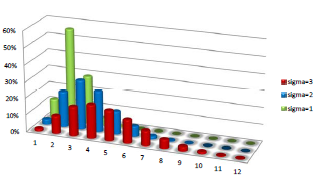
\includegraphics[width=0.5\textwidth]{images/Simulation/Rayleighverteilung.png}\\\\
Gemäss Formel braucht es für die Berechnung der Rayleigh-Verteilung zwei normalverteilte Zahlen.
\lstinputlisting[language=C++]{code/Rayleighmethode.cpp}

\subsection{Schlussbetrachtung}
\begin{itemize}
	\item Je nach Anwendungsgebiet sind für reproduzierbare Tests unterschiedliche Verteilungen angebracht.
	\item Mit den vorgestellten Werkzeugen sind die Grundlagen dafür geschaffen.
	\item Die Reproduzierbarkeit wird erreicht durch
	\begin{itemize}
		\item Pseudo-Zufallszahlengenerator
		\item Definiertem Random Seed
	\end{itemize}
	\item Beim Umwandeln einer Floating Point-Zahl in eine ganze Zahl muss überlegt werden, ob Runden (rounding) oder Abschneiden (truncating) die richtige Metode ist.
\end{itemize}

\subsubsection{Templateklassen}
\begin{itemize}
	\item C++ bietet ab C++11 in $<$random$>$ verschiedene Templateklassen an
	\begin{itemize}
		\item \textbf{Uniform distributions}\\ uniform\_int\_distribution, uniform\_real\_distribution
		\item \textbf{Bernoulli distributions}\\ bernoulli\_distribution, binomial\_distribution, negative\_binomial\_distribution, geometric\_distribution
		\item \textbf{Poisson distribution}\\ poisson\_distribution, exponential\_distribution, gamma\_distribution, weibull\_distribution, extreme\_value\_distribution
		\item \textbf{Normal distributions}\\ normal\_distribution, lognormal\_distribution, chi\_squared\_distribution, cauchy\_distribution, fisher\_f\_distribution, student\_t\_distribution
		\item \textbf{Sampling distributions}\\ discrete\_distribution, piecewise\_constant\_distribution, piecewise\_linear\_distribution
	\end{itemize}
\end{itemize}
